\documentclass{article}
\usepackage[utf8]{inputenc}
\usepackage[]{graphicx}


\title{User Guide for GB Polymer Model in LAMMPS}
\author{David Friday, Alex Cohen, Nick Jackson \\ friday1@illinois.edu, aecohen@mit.edu, jacksonn@illinois.edu}

\begin{document}

\maketitle

\section{Introduction}
Welcome to the user guide for the GB polymer model in LAMMPS. This polymer model can be used to model and simulate diverse anisotropic polymers with varying degrees of coarse-graining. The attached files include codes for generating LAMMPS data files and input scripts, submitting data files, and analyzing and visualizing the results from the simulations. The code is intended to be automated and easy-to-use. Thus, the user needs to specify only a small number parameters before running the codes. We believe that this model provides essential insights into anisotropic polymer structural and dynamical properties with enough specificity as to differentiate between different polymer chemistries. We hope this model proves useful in your research!

\section{How to Anisotropic CG Code with LAMMPS}
Before generating the LAMMPS executable, we need to edit the LAMMPS source code to contain the functionality for the dihedrals. Copy and paste the bond\_eldihedral.cpp and bond\_eldihedral.h files into the \textbf{ASPHERE} directory (which is within the \textbf{src} directory) in the LAMMPS source code. \textbf{Note: the dihedral vector is associate with the second diameter of the ellipsoids.}
In order to generate a LAMMPS executable with the appropriate packages installed, you will need to run the cmake command with the following specifications:

cmake -D PKG\_REPLICA=on -D PKG\_MISC=on -D PKG\_ASPHERE=on -D PKG\_MOLECULE=on -D PKG\_BODY=on -D PKG\_RIGID=on -D BUILD\_MPI=yes -D BUILD\_OMP=yes

\section{How to Prepare Data files}
The files provided allow you to generate LAMMPS data files with a minimal number of user input parameters. These parameters include the structure of a single monomer, the degree of polymerization, the number of polymers in the simulation box, the polymer spacing, and the box dimensions. While reading the following explanations, it may be helpful to consult an example .mon file with a schematic of its corresponding polymer in Figures \ref{fig:mon_file} - \ref{fig:polymer}. 

The first step for preparing a data file is to create a .mon file that includes the structure of a single monomer. The .mon file has four sections: Particles, Angles, Dihedrals/Bonds, and Rigid. Each section must begin with a single line that contains the name of the section followed by a colon, with no spaces. Specifically, the particles section must begin with a line containing only "Particles:", the angles section must begin with a line containing only "Angles:", the dihedrals/bonds section must begin with a line containing only "Dihedrals/Bonds:", and the rigid section must begin with a line containing only "Rigid:". The sections must also be specified in the order described above. The structure of information required in each section is outlined below. We have also provided a sample .mon file for a coarse-grained polymer and an image of the polymer with each particle numbered and certain parameters visually explained. It may be helpful to follow along with this image and the .mon file while trying to understand the information below. 

\subsection{Particles}
The particles section contains information about the spatial arrangement and intrinsic features of the coarse-grained particles in the monomer. Each line in the particles section must correspond to the following format, where each component is separated by a single space:

Particle Number, Particle Type, X Position, Y Position, Z Position, Charge, Ellipsoid Flag, Density, X Diameter, Y Diameter, Z Diameter

The X,Y,Z positions are relative to an arbitrary starting position. The ellipsoid flag variable specifies whether the particle is an ellipsoid (in which can it should contain "1") or a point particle (in which case it should contain "0"). If the particle is an ellipsoid, the Density value is a true density. If the particle is a point particle, the Density value corresponds to the mass of the point particle. In addition, point particles must contain zeros for the three diameter values. Usually, all particles are ellipsoids except for the bond sites, which are point particles with very small masses relative to the masses of the ellipsoids. 


\begin{figure}
\centering
    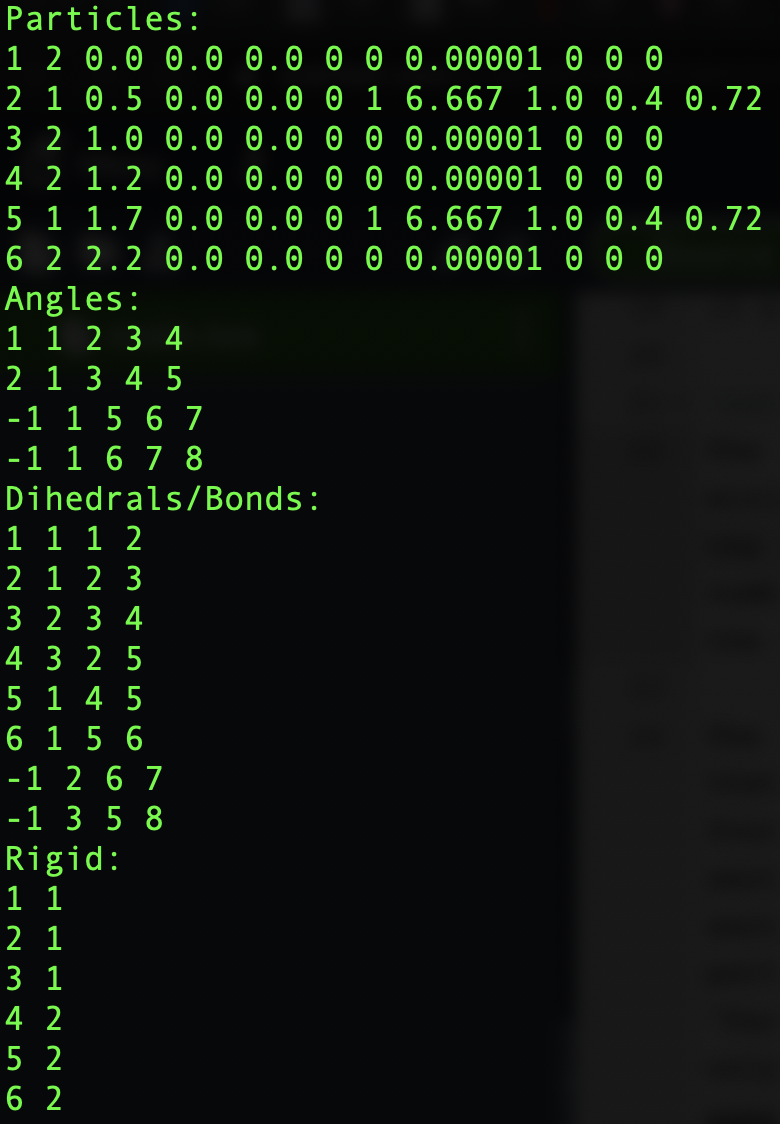
\includegraphics[width=.6\linewidth]{example_monfile.png}
    \caption{Example monomer file containing all necessary sections and formatting.}
    \label{fig:mon_file}
\end{figure}

\begin{figure}
\centering
    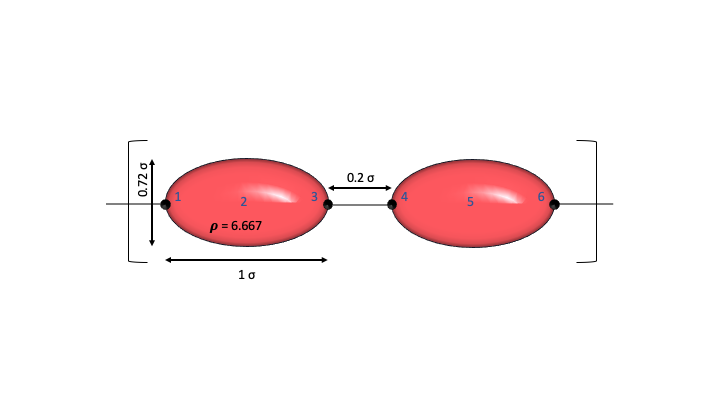
\includegraphics[width=.8\linewidth]{example_polymer.png}
    \caption{Schematic of monomer corresponding to the monomer file and input script included in this package.}
    \label{fig:polymer}
\end{figure}

\subsection{Angles}
The angles section contains information about the angle potentials that are specified in every monomer. Each line in the angles section must correspond to the following format, where each component is separated by a single space:

Angle Number, Angle Type, Particle Number of first particle in angle, Particle Number of middle particle in angle, Particle Number of third particle in angle

We also note that in many cases, there will be angles defined across monomers. For example, a simple coarse-grained anisotropic polymer consisting of disks connected by harmonic bonds will have angles defined between the disks down the backbone of the polymer chain. In order to specify one of these angles that crosses the monomer boundary, a "-1" must be placed where the Angle Number usually resides. In addition, the particles that are included in the angle that are in the "next monomer" (and are therefore not specified in the particles section) must be given the number that the will correspond to in the actual polymer (this number will equal the particle number of the corresponding particle in the specified monomer plus the total number of specified particles in the .mon file).

\subsection{Dihedrals/Bonds}
The dihedrals/bonds section contains information about the dihedral and bond potentials that are specified in every monomer. Dihedrals and bonds are lumped together because the dihedrals between two ellipsoids have been implemented using the bonds feature in LAMMPS. Each line in the dihedrals/bonds section must correspond to the following format, where each component is separated by a single space:

Dihedral/Bond Number, Dihedral/Bond Type, Particle Number of first particle in the dihedral/bond, Particle Number of second particle in the dihedral/bond

Similar to the angles, there will be dihedrals and bonds that exist across monomers in many cases. For example, every polymer will have a bond defined between two monomers. These dihedrals and bonds that span across two monomers must contain a "-1" in the Dihedral/Bond Number spot. The particle numbers are then specified in the same way as the particle numbers in the angles section are specified.

\subsection{Rigid}
The rigid section contains information about the rigid bodies that are specified in every monomer. Each line in the rigid section must correspond to the following format, where each component is separated by a single space:

Particle Number, Rigid Body Number

If the particle is not a part of any rigid body, 0 can be placed in the spot for Rigid Body Number (although, in reality, any number should work).

Note: For simple polymers that contain no internal angles and dihedrals, you may need to include information about two monomers in your .mon file. The data the user then provides in the script to produce the actual LAMMPS data file, which is outlined below, must be adjusted accordingly.

\subsection{Data file production script}
The data file production script, named datafile\_production.py, contains the code to generate the actual LAMMPS data file from the monomer file. There are 9 variables located at the top of the datafile\_production.py that the user must specify. These variables are:
\begin{enumerate}
    \item NUM\_MOLECULES = total number of polymers in the simulation
    \item NUM\_MONOMERS = total number of monomers per polymer (degree of polymerization)
    \item monomerOffset = distance between a particle in one monomer to the corresponding particle in the next monomer
    \item moleculeOffset = distance to separate different polymers by
    \item mon\_file\_name = name of monomer information file
    \item data\_file\_name = name of the output data file
    \item box\_x = length of box in x direction
    \item box\_y = length of box in y direction
    \item box\_z = length of box in z direction
\end{enumerate}

In order to create the data file, the monomer information file and
\newline
datafile\_production.py must be located in the same directory. The resulting data file will also be placed in this same directory.

\section{How to Prepare input files}
Input files define the interactions between the different types of particles as well as the simulation details. I will not go into the details of how to set it up, as extensive instructions can be found on the LAMMPS website. I have included a sample input file along with this user guide.

\section{How to Analyze Output}
Analysis will depend on what you are specifically interested in studying. In my case, I was interested in simple polymer structural properties, such as radius of gyration, order parameters along the stacking and bond axis, and RDFs. The analysis scripts that you will write to calculate properties of interest will depend on the way you have formatted the LAMMPS output files. 

For reference, I have included six python scripts that accomplish some of the basic analysis listed above. The analysis scripts require the data to be formatted according to the LAMMPS output files in the submit\_generator.py script. The six python scripts are described below:
\begin{enumerate}
    \item replica\_rg\_compilation.py. Generates a file containing the values of the radius of gyration at each time step for each temperature.
    \item replica\_traj\_compilation.py. Compiles the trajectory data into new files where each file corresponds to a specific temperature. (This is needed because LAMMPS will output the data such that each file corresponds to a processor, but the swaps change the temperature assigned to each processor -- see LAMMPS website for more information.)
    \item replica\_op\_compilation\_bond.py. Creates a file for each temperature which contains the order parameter along the bond axis at each time step.
    \item replica\_op\_compilation\_stacking.py. Creates a file for each temperature which contains the order parameter along the stacking axis at each time step.
    \item replica\_op\_onefile\_bond.py. Compiles all of the files created by \newline replica\_op\_compilation\_bond.py into one file.
    \item replica\_op\_onefile\_stacking.py. Compiles all of the files created by \newline replica\_op\_compilation\_stacking.py into one file.
\end{enumerate}

\section{How to Visualize Output in OVITO}
First, create a new .mon file which is the exact same as before except now only include the bonds that you want to visualize (and renumber the bonds). Next, run the datafile\_viz.py script, using the same parameters as used in the datafile\_production.py script. Then, run the conjugated\_visualization.py script, where the ell variable contains the file name for the trajectory file which contains the real particles and the all\_atoms variable contains the file name for the trajectory file which contains all particles. Load the data file (output of datafile\_viz.py) into ovito. Then click \textbf{Add modification...} in the top right and click \textbf{Load trajectory} under the \textbf{Modification heading}. Then, load the trajectory file (output of conjugated\_visualization.py) in the \textbf{Trajectory Source: External file} section on the right. To make the ellipsoids have the correct orientation, click \textbf{Edit column mapping...} in the bottom right. Set the \textbf{Particle property} of c\_op[1], c\_op[2], c\_op[3], and c\_op[4] to \textbf{Orientation}. Then, set the \textbf{Component} of c\_op[1], c\_op[2], c\_op[3], and c\_op[4] to \textbf{X}, \textbf{Y}, \textbf{Z}, \textbf{W}, respectively (Note: this may change if you change the LAMMPS output). 

\section{My Workflow}
To give you a sense of how I ran all of the simulations to generate all of the data, I will briefly discuss my workflow. First, I would draw out a diagram of what I wanted the monomer to look like, similar to Figure \ref{fig:polymer}. Next, I would translate this image into a .mon file similar to Figure \ref{fig:mon_file}. I would then run the datafile\_production.py script to generate the LAMMPS data file. I would then create a LAMMPS input script for running a simulation of a single polymer chain at a single temperature (see in.initialize). This input script would be used to run the chain at a high temperature, generating restart files that I can use as starting trajectories for my replica exchange simulations. Once this simulation is complete, I would modify the submit\_generator.py script to contain the correct parameters for my replica exchange runs. I would then run submit\_generator.py to collect data. 

\section{LAMMPS Notes}
Do not include a minimize command in the LAMMPS input script. It is incompatible with the rigid command, and the ghost particles will move. Instead, use a large langevin damping parameter for a short period of time to let the system slowly equilibrate. 

\end{document}
